%\documentclass[border=2pt]{article}
\documentclass[convert={density=300,size=1080x800,outext=.png}]{standalone}
\usepackage[utf8]{inputenc}
\usepackage{tikz}

\begin{document}
 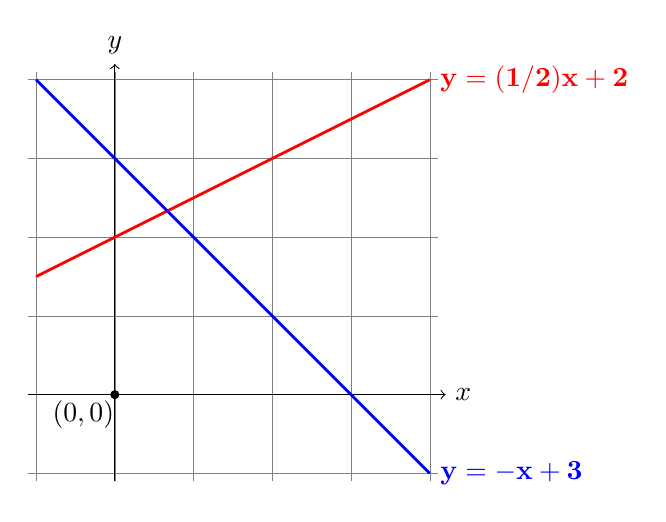
\begin{tikzpicture}[domain=-1:4] 
	   \draw[very thin,color=gray] (-1.1,-1.1) grid (4.1,4.1);
	   \draw[->] (-1.1,0) -- (4.2,0) node[right] {$x$}; 
	   \draw[->] (0,-1.1) -- (0,4.2) node[above] {$y$};
	   \draw[color=red, line width=1.0]    plot (\x,{0.5 * \x + 2})             node[right] {$\mathbf{y = (1/2) x + 2}$};
	   \draw[color=blue, line width=1.0]    plot (\x,{-1 * \x + 3})             node[right] {$\mathbf{y = -x + 3}$};
	   \node at (-0.4,-0.25) {$(0, 0)$};
	   \draw [color=black, fill=black] (0, 0) circle (0.05); 
 \end{tikzpicture}
\end{document}


	%	\addplot[red,  ultra thick] (x, );
	%	\draw[red] (-1,-1) node[right] {$$ $$};
	%
	%	\addplot[blue, ultra thick] (x, -1 * x + 5);
	%	\draw[blue] (600,9) node[right] {$$ Y = -X + 5$$};
	%		\draw[thick,->] (0,0) -- (4.5,0) node[anchor=north west] {x axis};
	%		\draw[thick,->] (0,0) -- (0,4.5) node[anchor=south east] {y axis};